\chapter{Especificação e Modelação}
\label{cha:especificacao_modelacao}

Neste capítulo, são detalhadas as especificações técnicas da solução desenvolvida. A análise de requisitos é apresentada em primeiro lugar, seguida pela modelação da arquitetura, da base de dados e da API, que em conjunto definem a estrutura e o comportamento do sistema.

\section{Análise de Requisitos}

A tabela seguinte resume os requisitos funcionais (RF) e não-funcionais (RNF) identificados para o projeto, juntamente com o estado final da sua implementação.

% Tabela de Requisitos atualizada
\begin{longtable}{|p{0.08\textwidth}|p{0.48\textwidth}|p{0.12\textwidth}|p{0.25\textwidth}|}
    \caption{Tabela de Requisitos e Estado de Implementação.} \label{tab:requisitos} \\
    \hline
    \textbf{ID} & \textbf{Descrição} & \textbf{Estado} & \textbf{Notas} \\
    \hline
    \endfirsthead
    
    \multicolumn{4}{c}%
    {{\bfseries \tablename\ \thetable{} -- continuação da página anterior}} \\
    \hline
    \textbf{ID} & \textbf{Descrição} & \textbf{Estado} & \textbf{Notas} \\
    \hline
    \endhead
    
    \hline \multicolumn{4}{|r|}{{Continua na página seguinte...}} \\ \hline
    \endfoot
    
    \hline
    \endlastfoot
    
    \multicolumn{4}{|c|}{\textbf{Requisitos Funcionais}} \\
    \hline
    RF1 & Suporte à importação de dados (CSV, JSON) & Cumprido & Implementada importação de mensagens via CSV e anotações via JSON. \\
    \hline
    RF2 & Organização de dados por projetos & Cumprido & Estrutura central da aplicação. \\
    \hline
    RF3 & Exportação dos dados anotados (JSON) & Cumprido & Funcionalidade de exportação por sala de chat implementada. \\
    \hline
    RF4 & Interface de utilizador clara e funcional & Cumprido & Interface React desenvolvida com foco na usabilidade para anotação. \\
    \hline
    RF5 & Suporte a múltiplos anotadores por projeto & Cumprido & Sistema de atribuição de utilizadores a projetos. \\
    \hline
    RF6 & Gestão de atribuição de tarefas & Cumprido & Administradores podem atribuir/remover utilizadores de projetos. \\
    \hline
    RF7 & Interface especializada para chat disentanglement & Cumprido & Ecrã de anotação dedicado com gestão de threads. \\
    \hline
    RF8 & Sistema de tagging para classificação em threads & Cumprido & Funcionalidade nuclear da anotação. \\
    \hline
    RF9 & Visualização sequencial das mensagens & Cumprido & A sala de chat apresenta as mensagens por ordem. \\
    \hline
    RF10 & Armazenamento para cálculo de métricas & Cumprido & O modelo de dados permite o cálculo de IAA. \\
    \hline
    RF11 & Autenticação de utilizadores & Cumprido & Implementado com JWT (access e refresh tokens). \\
    \hline
    RF12 & Definição de roles (admin/anotador) & Cumprido & O modelo `User` contém o campo `is\_admin`. \\
    \hline
    RF13 & Controlo de acesso baseado em permissões & Cumprido & Endpoints da API protegidos com base no role. \\
    \hline
    \multicolumn{4}{|c|}{\textbf{Requisitos Não Funcionais}} \\
    \hline
    RNF1 & Tempo de resposta adequado & Cumprido & A API responde rapidamente a pedidos interativos. \\
    \hline
    RNF2 & Processamento eficiente para múltiplos utilizadores & Parcialmente & A arquitetura suporta-o, mas não foram feitos testes de carga formais. \\
    \hline
    RNF3 & Interface responsiva & Parcialmente & O design é funcional mas não foi totalmente otimizado para todos os tamanhos de ecrã. \\
    \hline
    RNF4 & Feedback visual claro & Cumprido & A interface React fornece feedback sobre o estado (loading, error, success). \\
    \hline
    RNF5 & Interface simples e intuitiva & Cumprido & O design focou-se na simplicidade para a tarefa de anotação. \\
    \hline
    RNF6 & Backup automático de anotações & Não Cumprido & Não implementado. Requer uma solução de infraestrutura (e.g., cron jobs na base de dados). \\
    \hline
    RNF7 & Logging de atividades críticas & Parcialmente & O backend utiliza logging básico, mas não um sistema de logging estruturado e exaustivo. \\
    \hline
\end{longtable}

\section{Modelação da Solução}

A modelação da solução foi um processo iterativo que resultou numa arquitetura cliente-servidor, um modelo de dados relacional bem definido e uma API RESTful estruturada.

\subsection{Arquitetura da Solução}

A plataforma segue uma arquitetura cliente-servidor desacoplada, composta por dois componentes principais:

\begin{itemize}
    \item \textbf{Frontend (Cliente):} Uma Single-Page Application (SPA) desenvolvida com a biblioteca \textbf{React}. É responsável exclusivamente pela apresentação da interface do utilizador e pela gestão do estado local da UI. Toda a lógica de negócio e manipulação de dados é delegada ao backend através de chamadas à API.
    \item \textbf{Backend (Servidor):} Uma API RESTful desenvolvida com a framework \textbf{FastAPI} (Python). É responsável por toda a lógica de negócio, incluindo a autenticação de utilizadores, controlo de permissões, operações na base de dados (CRUD) e cálculos de métricas como o IAA.
\end{itemize}
Esta separação estrita de responsabilidades (`separation of concerns`) garante uma maior manutenibilidade, escalabilidade e a possibilidade de desenvolver e testar os dois componentes de forma independente.

\subsection{Modelo de Dados}

O coração do backend é o seu modelo de dados relacional, implementado com \textbf{SQLAlchemy} como ORM (Object-Relational Mapper), que mapeia as classes Python para tabelas numa base de dados SQLite. A Figura~\ref{fig:modelo-er} apresenta o Diagrama de Entidade-Relação (ERD) final do sistema.

As entidades centrais do modelo são:
\begin{itemize}
    \item \textbf{User, Project, e ProjectAssignment:} que em conjunto gerem os utilizadores e as suas permissões de acesso aos diferentes projetos.
    \item \textbf{ChatRoom e ChatMessage:} que estruturam os dados a serem anotados.
    \item \textbf{Annotation:} a tabela principal que armazena a ligação entre uma mensagem, um anotador e um \textit{thread}, sendo a base para toda a análise posterior.
\end{itemize}
A utilização do SQLAlchemy e do Alembic para migrações de base de dados permitiu uma evolução estruturada do esquema ao longo do desenvolvimento do projeto.

\subsection{API RESTful}

A comunicação entre o frontend e o backend é realizada através de uma API RESTful. A API expõe um conjunto de endpoints para todas as operações necessárias, desde a autenticação até ao cálculo de métricas. A API está documentada seguindo o standard OpenAPI, o que facilita a sua exploração e integração.

Os endpoints estão logicamente agrupados por responsabilidade:
\begin{itemize}
    \item \textbf{Auth:} Gestão de autenticação e tokens.
    \item \textbf{Projects:} Operações de utilizador normal sobre projetos e salas de chat.
    \item \textbf{Annotations:} Criação e gestão de anotações.
    \item \textbf{Admin:} Operações de administração, incluindo importação/exportação e cálculo de IAA.
\end{itemize}

\section{Protótipos de Interface}

\subsection{Mapa de Navegação}

A estrutura de navegação da plataforma está concebida para se adaptar aos diferentes perfis de utilizador. O sistema prevê um portal de login onde, após autenticação, os utilizadores terão acesso a um dashboard principal, que funcionará como ponto central de acesso às diversas funcionalidades da plataforma. A estrutura completa do mapa de navegação pode ser visualizada na Figura~\ref{fig:mapa-navegacao}.

A ferramenta de anotação poderá ser estruturada de forma a acomodar diferentes tipos de tarefas no futuro, onde o dashboard principal permitirá acesso às várias funcionalidades disponíveis. Numa primeira fase, a funcionalidade de \textit{disentanglement} constitui o foco principal da implementação.

\subsection{Principais Interfaces}

\subsubsection{Portal de Entrada}
O acesso à plataforma é controlado através de um portal de autenticação minimalista. Esta decisão de design visa garantir a integridade dos dados e a atribuição correta das tarefas de anotação, sendo o login obrigatório para qualquer interação com os dados do sistema.

\subsubsection{Dashboard Principal}
Após autenticação, o utilizador acede a um dashboard que apresenta uma visão geral da plataforma. Este componente central adapta-se dinamicamente ao perfil do utilizador (administrador ou anotador), apresentando as funcionalidades relevantes e o estado atual das tarefas atribuídas.

\subsubsection{Funcionalidade de Disentanglement}
A funcionalidade principal implementada na plataforma foca-se na tarefa de \textit{disentanglement} de chat, apresentando duas visões distintas:

\paragraph{Visão do Anotador}
Para os anotadores, a interface apresenta:
\begin{itemize}
    \item Lista das chatrooms atribuídas automaticamente pelo sistema
    \item Interface de anotação com visualização sequencial das mensagens
    \item Sistema intuitivo de tagging para classificação de threads
    \item Indicadores de progresso da tarefa
    \item Mecanismos de validação em tempo real
\end{itemize}

\paragraph{Visão do Administrador}
Os administradores têm acesso a funcionalidades adicionais:
\begin{itemize}
    \item Gestão completa dos datasets
    \item Monitorização do progresso dos anotadores
    \item Visualização de métricas e estatísticas
    \item Configuração da distribuição automática de tarefas
\end{itemize}

\subsubsection{Interface de Anotação}
O componente central da funcionalidade de \textit{disentanglement} é a interface de anotação, que foi concebida para maximizar a eficiência do processo de anotação. Cada chatroom é apresentada como uma sequência temporal de mensagens, onde o anotador pode facilmente:
\begin{itemize}
    \item Visualizar o contexto completo da conversa
    \item Criar e atribuir tags de thread às mensagens
    \item Acompanhar o progresso da anotação em tempo real
    \item Navegar eficientemente entre diferentes chatrooms
\end{itemize}

O sistema mantém uma gravação automática do progresso, permitindo que os anotadores retomem o seu trabalho de forma contínua em qualquer momento.


\begin{figure}[p]
    \centering
    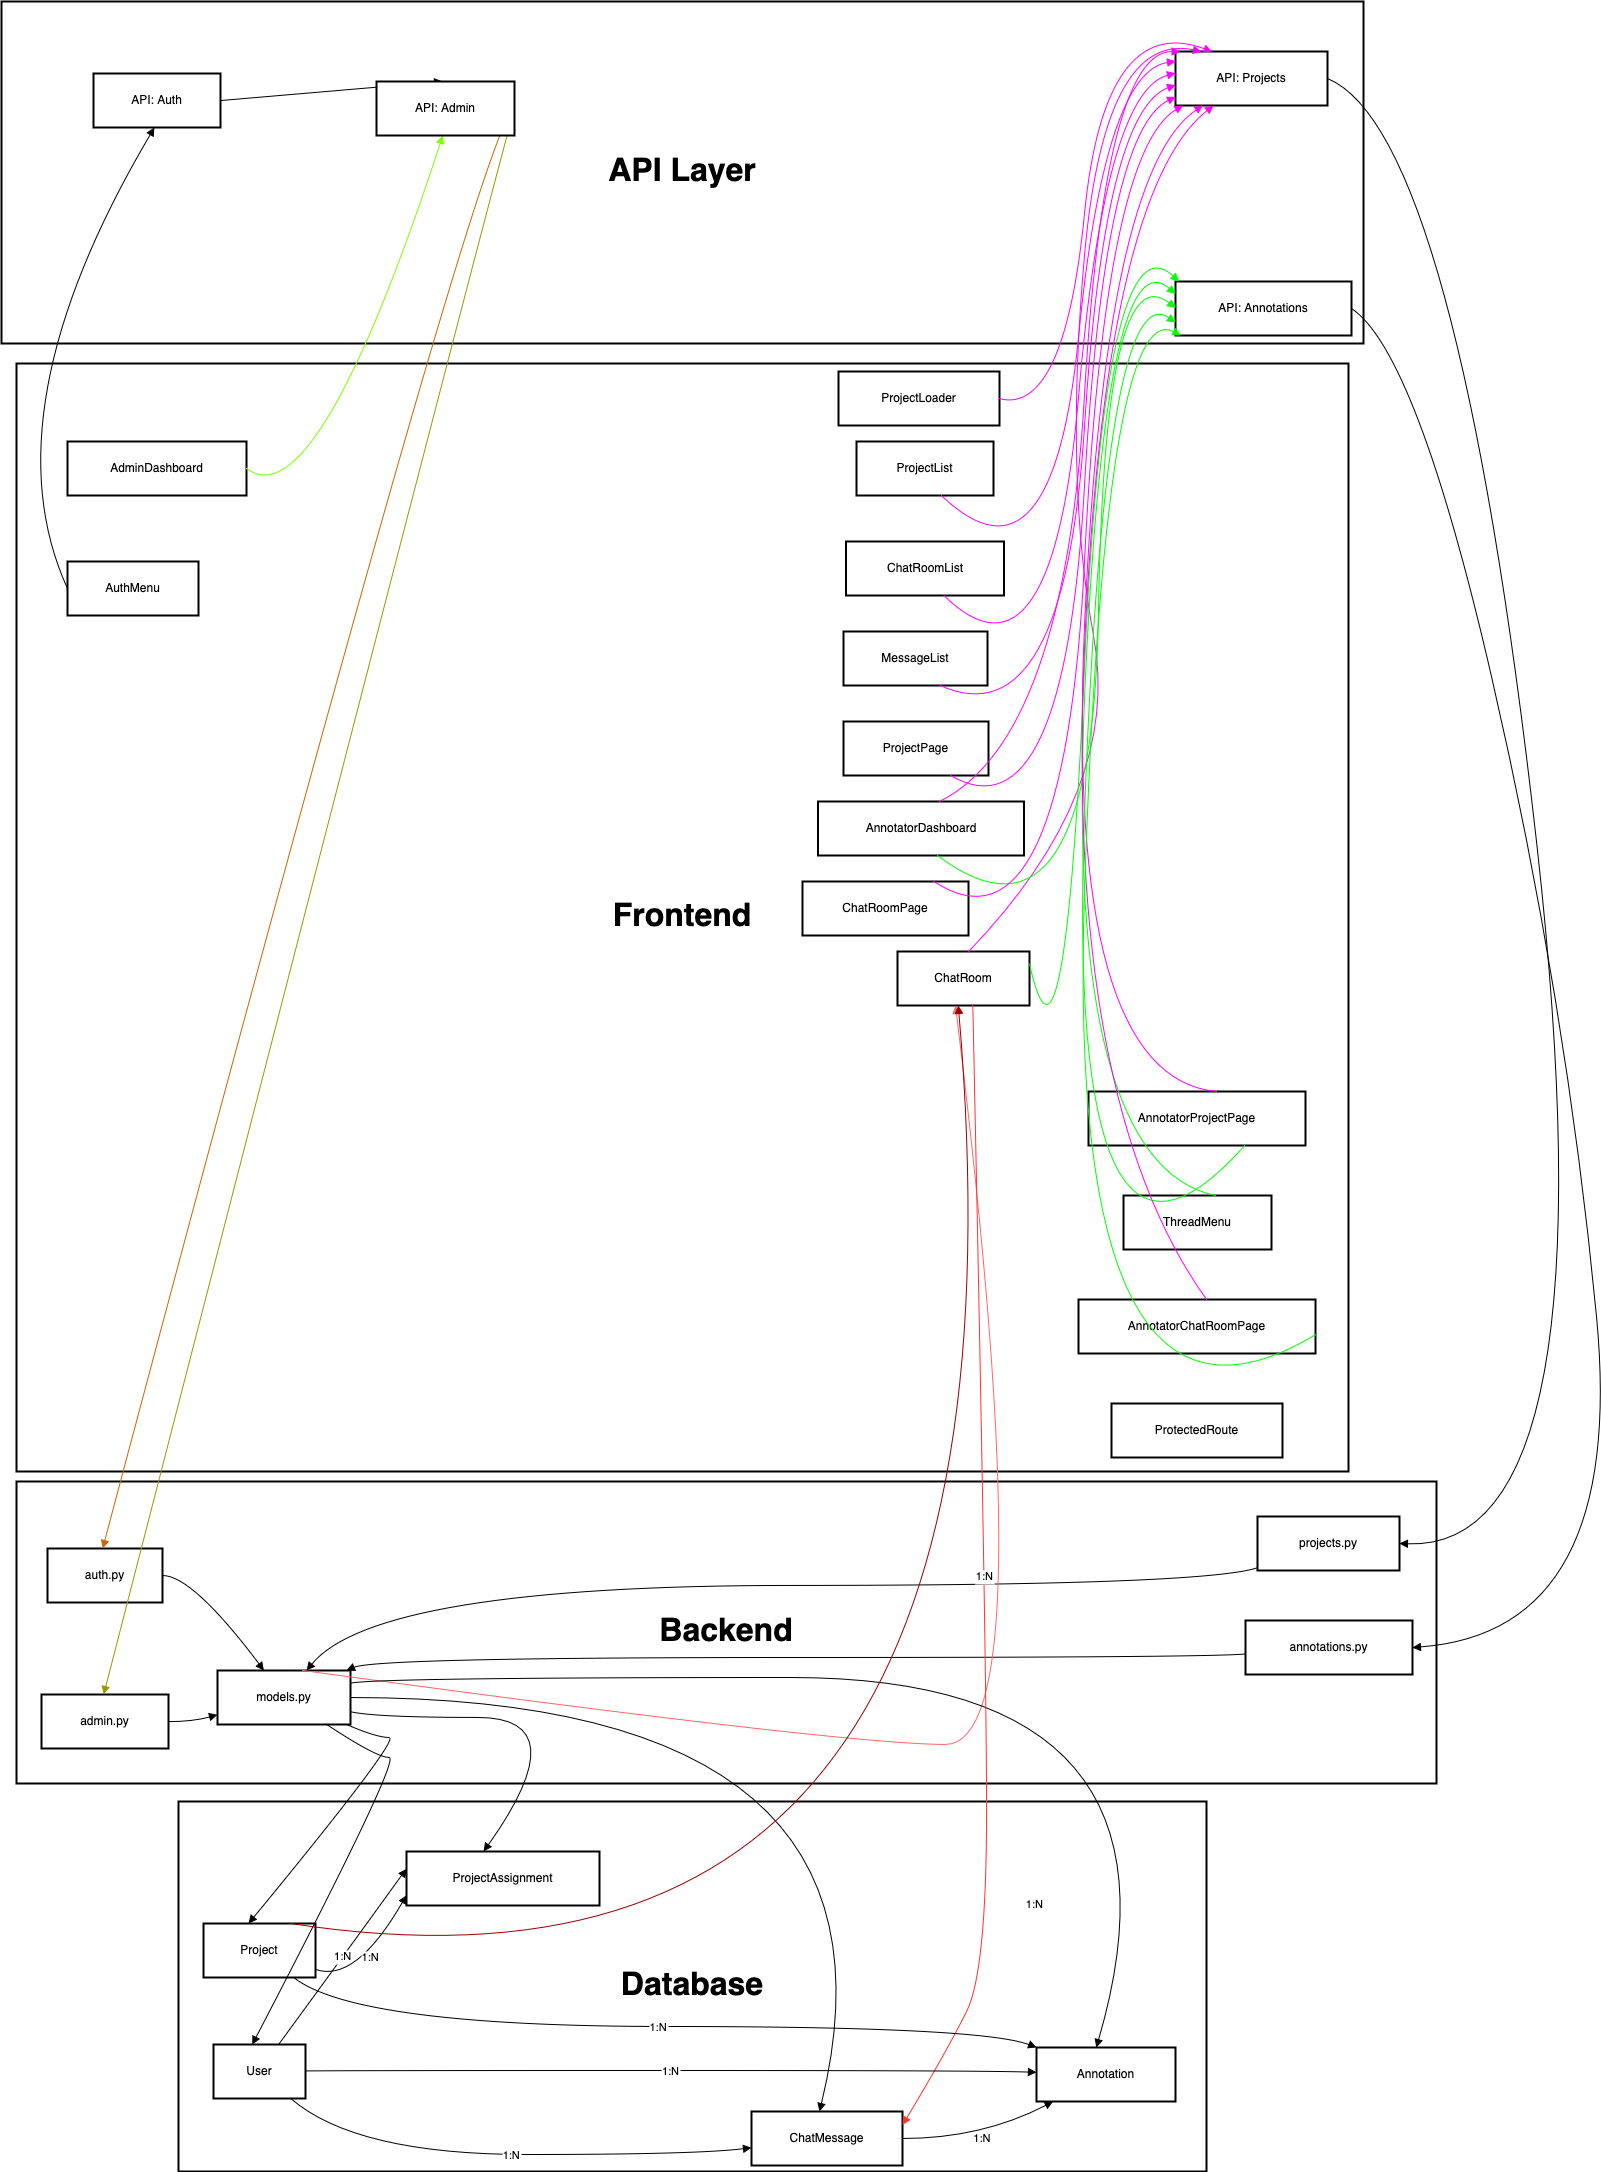
\includegraphics[width=0.95\textwidth,height=0.95\textheight,keepaspectratio]{images/2A-ERT-B.drawio.png}
    \caption{Modelo de Entidade-Relação final do Sistema.}
    \label{fig:modelo-er}
\end{figure}

\begin{landscape}
    \begin{figure}[p]
        \centering
        \makebox[\textwidth][c]{%
            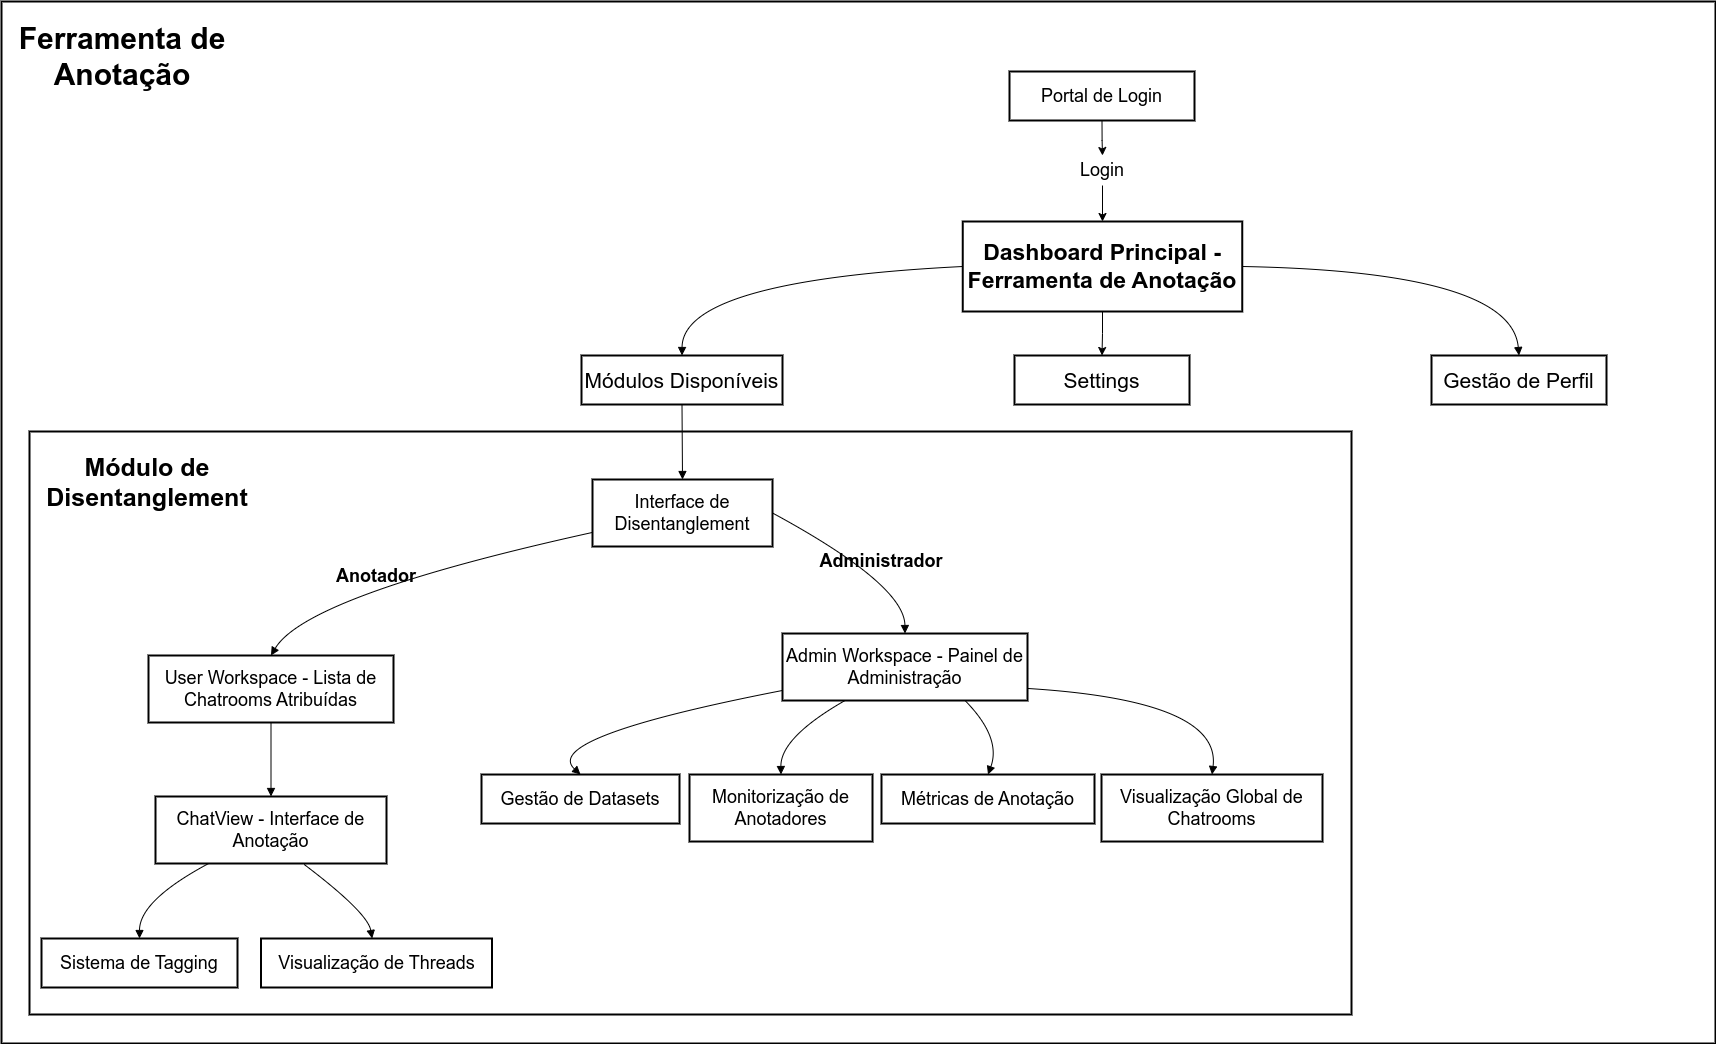
\includegraphics[width=0.8\paperheight, angle=0, keepaspectratio]{images/mapaDeNavegacaoSistema.drawio.png}
        }
        \caption{Mapa de Navegação do Sistema.}
        \label{fig:mapa-navegacao}
    \end{figure}
\end{landscape}